%%
%% Copyright 2007-2019 Elsevier Ltd
%%
%% This file is part of the 'Elsarticle Bundle'.
%% ---------------------------------------------
%%
%% It may be distributed under the conditions of the LaTeX Project Public
%% License, either version 1.2 of this license or (at your option) any
%% later version.  The latest version of this license is in
%%    http://www.latex-project.org/lppl.txt
%% and version 1.2 or later is part of all distributions of LaTeX
%% version 1999/12/01 or later.
%%
%% The list of all files belonging to the 'Elsarticle Bundle' is
%% given in the file `manifest.txt'.
%%
%% Template article for Elsevier's document class `elsarticle'
%% with harvard style bibliographic references

%\documentclass[preprint,12pt]{elsarticle}

%\textheight 230mm \textwidth 170mm \topmargin 0.5cm \oddsidemargin
%0pt \evensidemargin 0pt
%\parskip=2mm
%\voffset -2cm
%% Use the option review to obtain double line spacing
%\documentclass[preprint,review,12pt]{elsarticle}

%% Use the options 1p,twocolumn; 3p; 3p,twocolumn; 5p; or 5p,twocolumn
%% for a journal layout:
%\documentclass[final,1p,times]{elsarticle}
 %\documentclass[final,1p,times,twocolumn]{elsarticle}
\documentclass[final,3p,times]{elsarticle}
%% \documentclass[final,3p,times,twocolumn]{elsarticle}
%% \documentclass[final,5p,times]{elsarticle}
%% \documentclass[final,5p,times,twocolumn]{elsarticle}

%% For including figures, graphicx.sty has been loaded in
%% elsarticle.cls. If you prefer to use the old commands
%% please give \usepackage{epsfig}

%% The amssymb package provides various useful mathematical symbols
\usepackage{amssymb}
\usepackage{graphicx,setspace}
\usepackage{psfrag}
\usepackage{amsfonts}
\expandafter\let\csname equation*\endcsname\relax
\expandafter\let\csname endequation*\endcsname\relax
\usepackage{amsmath}
\usepackage{amssymb, amsthm}
\usepackage{mathrsfs}
\usepackage{epstopdf}
\usepackage{float}
\usepackage{lineno,hyperref}
\usepackage{color}
\usepackage{subfigure}

\usepackage{amsmath}
%\usepackage{amsthm}
\usepackage{dsfont} % it is the package of using the "\mathds{} "
\usepackage{amssymb} % it is the package of using the "\mathbb{}"
\usepackage{graphicx,color}
\usepackage{extarrows}

\bibliographystyle{elsarticle-num}
\usepackage{graphicx}

\usepackage{epstopdf}
%% The amsthm package provides extended theorem environments
%% \usepackage{amsthm}

%% The lineno packages adds line numbers. Start line numbering with
%% \begin{linenumbers}, end it with \end{linenumbers}. Or switch it on
%% for the whole article with \linenumbers.
%% \usepackage{lineno}

\journal{?}

\begin{document}
\newtheorem{definition}{Definition}[section]
\newtheorem{lemma}{Lemma}[section]
\newtheorem{remark}{Remark}[section]
\newtheorem{theorem}{Theorem}[section]
\newtheorem{proposition}{Proposition}
\newtheorem{assumption}{Assumption}
\newtheorem{example}{Example}
\newtheorem{corollary}{Corollary}[section]
\def\ep{\varepsilon}
\def\Rn{\mathbb{R}^{n}}
\def\Rm{\mathbb{R}^{m}}
\def\E{\mathbb{E}}
\def\hte{\hat\theta}
%\numberwithin{theorem}{section}
%\numberwithin{definition}{section}
\renewcommand{\theequation}{\thesection.\arabic{equation}}
\begin{frontmatter}

%% Title, authors and addresses

%% use the tnoteref command within \title for footnotes;
%% use the tnotetext command for theassociated footnote;
%% use the fnref command within \author or \address for footnotes;
%% use the fntext command for theassociated footnote;
%% use the corref command within \author for corresponding author footnotes;
%% use the cortext command for theassociated footnote;
%% use the ead command for the email address,
%% and the form \ead[url] for the home page:
%% \title{Title\tnoteref{label1}}
%% \tnotetext[label1]{}
%% \author{Name\corref{cor1}\fnref{label2}}
%% \ead{email address}
%% \ead[url]{home page}
%% \fntext[label2]{}
%% \cortext[cor1]{}
%% \address{Address\fnref{label3}}
%% \fntext[label3]{}




\title{Targeted Micro-Robots Locate Cancer Cells}


%% \author[label1,label2]{}
%% \address[label1]{}
%% \address[label2]{}

\author{Ruijie He\fnref{addr1,addr2}}\ead{gravitas_sysu@qq.com}
\author{Shenglan Yuan\corref{cor1}\fnref{addr1}}
\ead{shenglanyuan@gbu.edu.cn}\cortext[cor1]{Corresponding author}


\address[addr1]{\rm Department of Mathematics, School of Sciences, Great Bay University, Dongguan 523000, China }
\address[addr2]{\rm School of Mathematics,Sun Yat-sen University, Guangzhou 510275, China}








\begin{abstract}

\end{abstract}

\begin{keyword}

%% keywords here, in the form: keyword \sep keyword

%% PACS codes here, in the form: \PACS code \sep code

%% MSC codes here, in the form: \MSC code \sep code
%% or \MSC[2008] code \sep code (2000 is the default)

\end{keyword}

\end{frontmatter}

%% \linenumbers

%% main text
\section{Introduction}
This work is to address how targeted micro-robots carrying drugs locate cancer cells, we present a mathematical model based on chemotaxis-driven movement and ligand-receptor binding. The model consists of three key equations describing the chemoattractant concentration, free micro-robots, and bound micro-robots.




\section{Mathematical model}
We are going to model the targeted delivery of drugs by micro-robots to cancer cells. The key steps include three parts. The release of micro-robots in the bloodstream. The navigation of micro-robots towards the tumor site, which we assume is guided by a chemical gradient (chemotaxis) or other targeting mechanisms. The binding of micro-robots to cancer cells.

We will focus on chemotaxis as a primary mechanism. The mathematical model will involve diffusion of chemoattractants (chemical signals) from the tumor, movement of micro-robots towards higher concentrations of chemoattractants, and binding kinetics when micro-robots come in contact with cancer cells. We will model the system using partial differential equations (PDEs) for the chemoattractant concentration and the density of micro-robots.

The chemoattractant is produced by the tumor cells. We model its diffusion and decay:
\begin{equation*}
\frac{\partial c}{\partial t}=D_c\nabla^{2}c-kc+S(\textbf{x}),
\end{equation*}
where $c(\textbf{x},t)$ is the concentration of chemoattractant at position $\textbf{x}$ and time $t$, $D_c$ is the diffusion coefficient ($\text{0.1 mm}^2$/s) of the chemoattractant, $\nabla^{2}$ is the Laplacian operator in 3D, $k$ is the decay rate ($\text{0.01 s}^{-1}$), and $S(\textbf{x})$ is the tumor  source term located at some region (1.0 nM/s in tumor region).

The micro-robots move by chemotaxis and diffuse randomly due to blood flow and other factors. The equation for the free micro-robots (movement via chemotaxis) is
\begin{equation*}
\frac{\partial \rho}{\partial t}=D_{\rho}\nabla^{2}\rho-\nabla\cdot(\chi \rho \nabla c)-k_{b}\rho\delta_{\Omega_{T}}+k_{u}b,
\end{equation*}
where $\rho(\textbf{x},t)$ is the density of micro-robots at position $\text{x}$ and time $t$, $D_{\rho}$ is the diffusion coefficient ($\text{0.01 mm}^2$/s) of micro-robots, $\nabla$ is the gradient operator in 3D, $\chi$ is the chemotactic sensitivity ($\text{0.1 mm}^2$/nM$\cdot$s), $k_{b}$ is the binding rate ($\text{0.1 s}^{-1}$) to cancer cells (only in the tumor region $\Omega_{T}$), $k_{u}$ is the unbinding rate ($\text{0.01 s}^{-1}$) since we assume bound micro-robots can detach at a low rate, and $\delta_{\Omega_{T}}$ is the indicator function that equals to 1 inside tumor region $\Omega_{T}$, 0 otherwise.

The bound micro-robots attached to cancer cells satisfy
\begin{equation*}
\frac{\partial b}{\partial t}=k_{b}\rho\delta_{\Omega_{T}}-k_{u}b,
\end{equation*}
where $b(\textbf{x},t)$ the density of bound micro-robots.

\section{Numerical simulations}
\begin{figure}[h]
\begin{center}
  \begin{minipage}{2.13in}
\leftline{(a)}
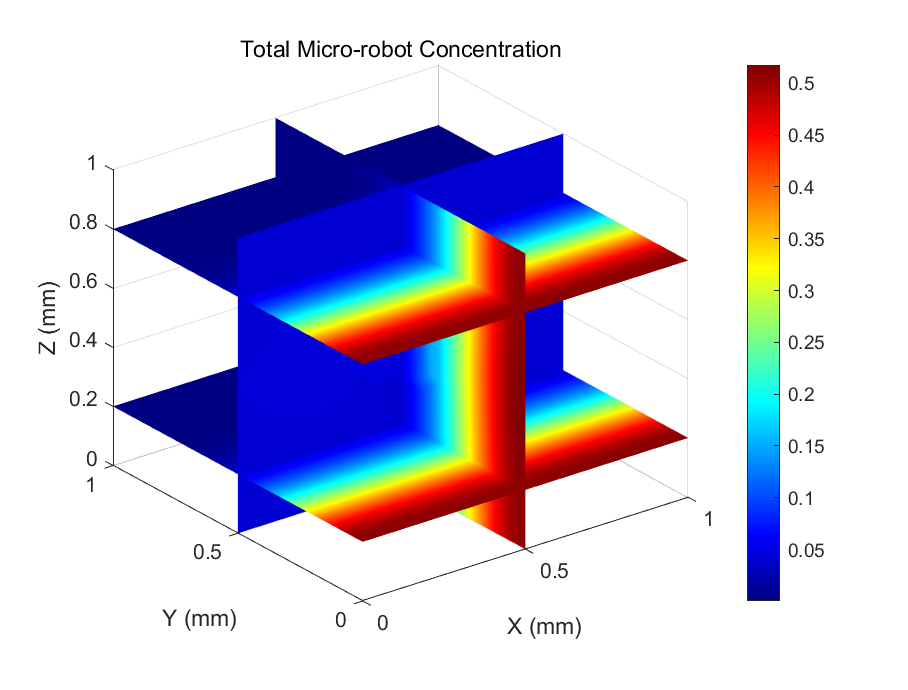
\includegraphics[width=2.13in]{TotalMRConcentration.eps}
\end{minipage}
\hfill
\begin{minipage}{2.13in}
\leftline{(b)}
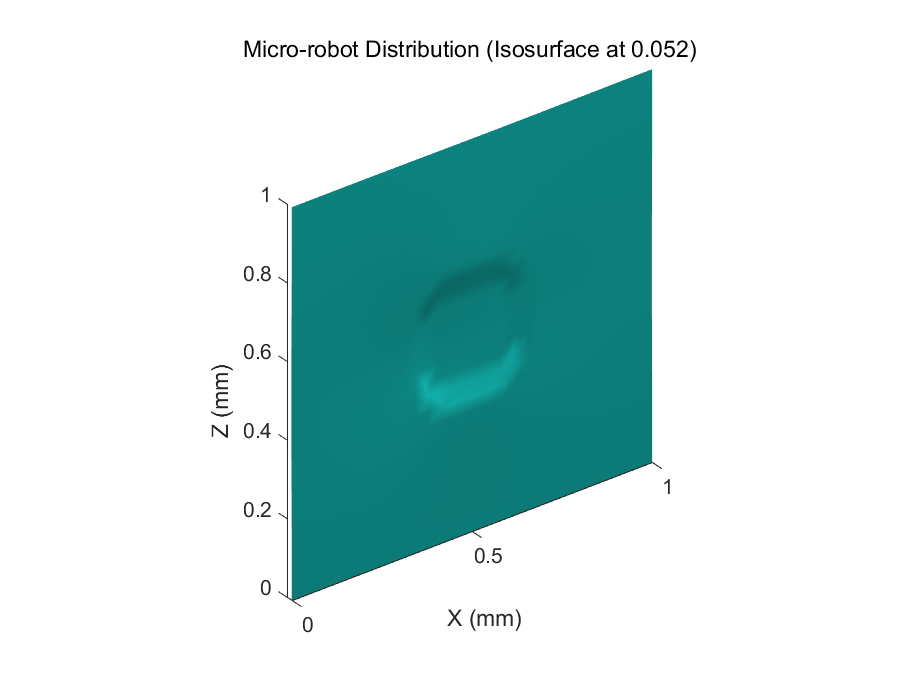
\includegraphics[width=2.13in]{MRDistribution.eps}
\end{minipage}
\hfill
  \begin{minipage}{2.13in}
\leftline{(c)}
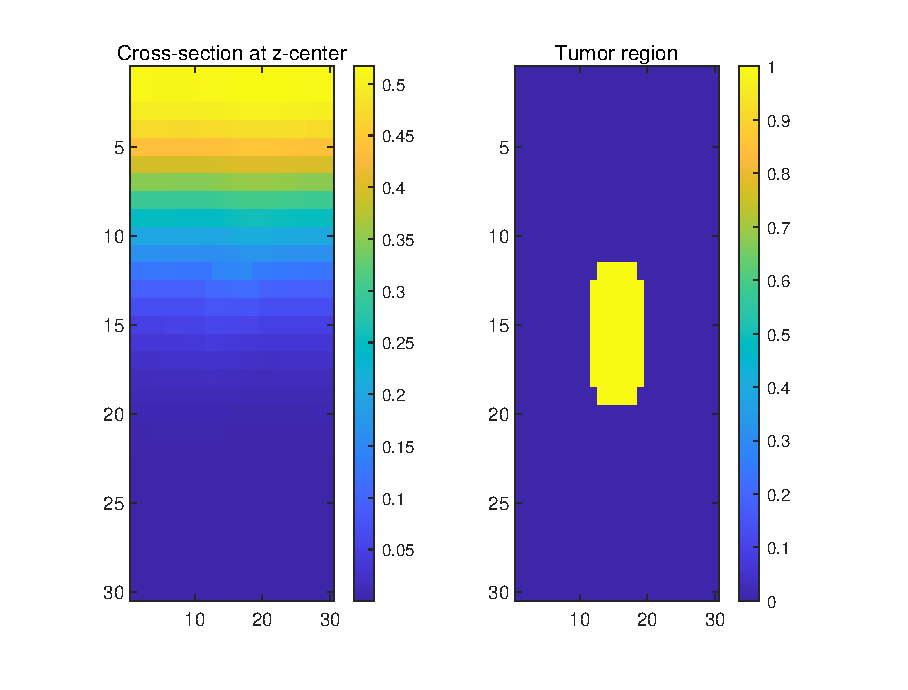
\includegraphics[width=2.13in]{TumorRegion.eps}
\end{minipage}
\caption{(a) Cross-sections of total robot concentration; (b) 3D surface at $10\%$ of max concentration; (c) 2D slices through domain center. }\label{ThreeDSim}
\end{center}
\end{figure}
Figure \ref{ThreeDSim} simulates a 3D chemotaxis-driven micro-robot drug delivery system. The simulation is configured within a $\text{1 mm}^{3}$ spatial domain, discretized with a grid of 30 points along each dimension. To ensure numerical stability, a time step of 0.001 seconds is used, and the total simulated time is 2 seconds. The key biochemical parameters governing the system include diffusivities for the chemoattractant and micro-robots ($D_c=0.1$ and $D_\rho=0.01$, respectively), a chemotactic sensitivity of $\chi=0.1$, and binding/unbinding rates of $k_b=0.2$ and $k_u=0.01$. The environment is initialized with a tumor modeled as a spherical region at the center with a radius of 0.15 mm, which acts as a continuous source of chemoattractant. The population of micro-robots is introduced into the system via an initial injection across the entire plane at $x=0$. At each time step of the simulation loop, zero-flux Neumann boundary conditions are enforced to contain all elements within the modeled domain. The chemoattractant field is updated by calculating its diffusion, incorporating a constant production term from the central tumor, and subtracting a natural decay term. Concurrently, the micro-robot population undergoes movement driven by a combination of random diffusion and a directed chemotactic velocity proportional to the spatial gradient of the chemoattractant ($\nabla c$), guiding them toward higher concentrations. Binding and unbinding kinetics, governed by their respective rates, are exclusively calculated for micro-robots located within the tumor region. Finally, after all updates are computed, the concentrations of all species are clipped to ensure non-negativity, maintaining physical realism before proceeding to the next iteration. We compute the 3D Laplacian using central differences, calculate the chemotaxis term $\nabla\cdot(\rho\nabla c)$, and implement zero-flux boundaries by copying adjacent grid values. Visualization of the simulation data is achieved through multiple complementary methods. A slice plot provides a cross-sectional view of the total micro-robot concentration, revealing internal gradients within the volume in Figure \ref{ThreeDSim}(a). To render the three-dimensional structure of the robot swarm, an isosurface is generated at a threshold of $10\%$ of the maximum concentration in Figure \ref{ThreeDSim}(b). Finally, for detailed quantitative analysis, 2D cross-sectional slices are extracted through the center of the domain and overlaid with a tumor mask to clearly distinguish the robotic population from the tumor region in Figure \ref{ThreeDSim}(c).
The simulation successfully models targeted drug delivery using chemotaxis, with robots accumulating in the tumor region due to binding and chemoattractant gradients.

\begin{figure}[H]
\vspace*{1pt}
\begin{center}
\begin{minipage}{5in}
		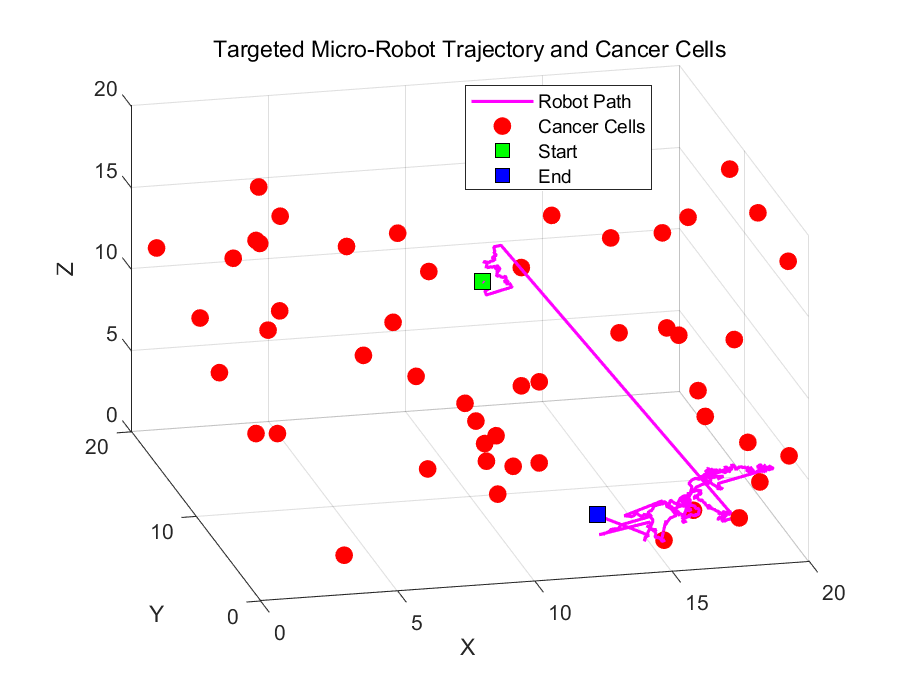
\includegraphics[width=5in]{simulateRobotAndCells.eps}
	\end{minipage}
\end{center}
\caption{}\label{SimulateRobotAndCells}	
\end{figure}


Figure \ref{SimulateRobotAndCells} clearly shows the robot's path, cell positions, and start/end points with appropriate markers and labels.


\begin{figure}[h]
\begin{center}
\begin{minipage}{4in}
\leftline{(a)}
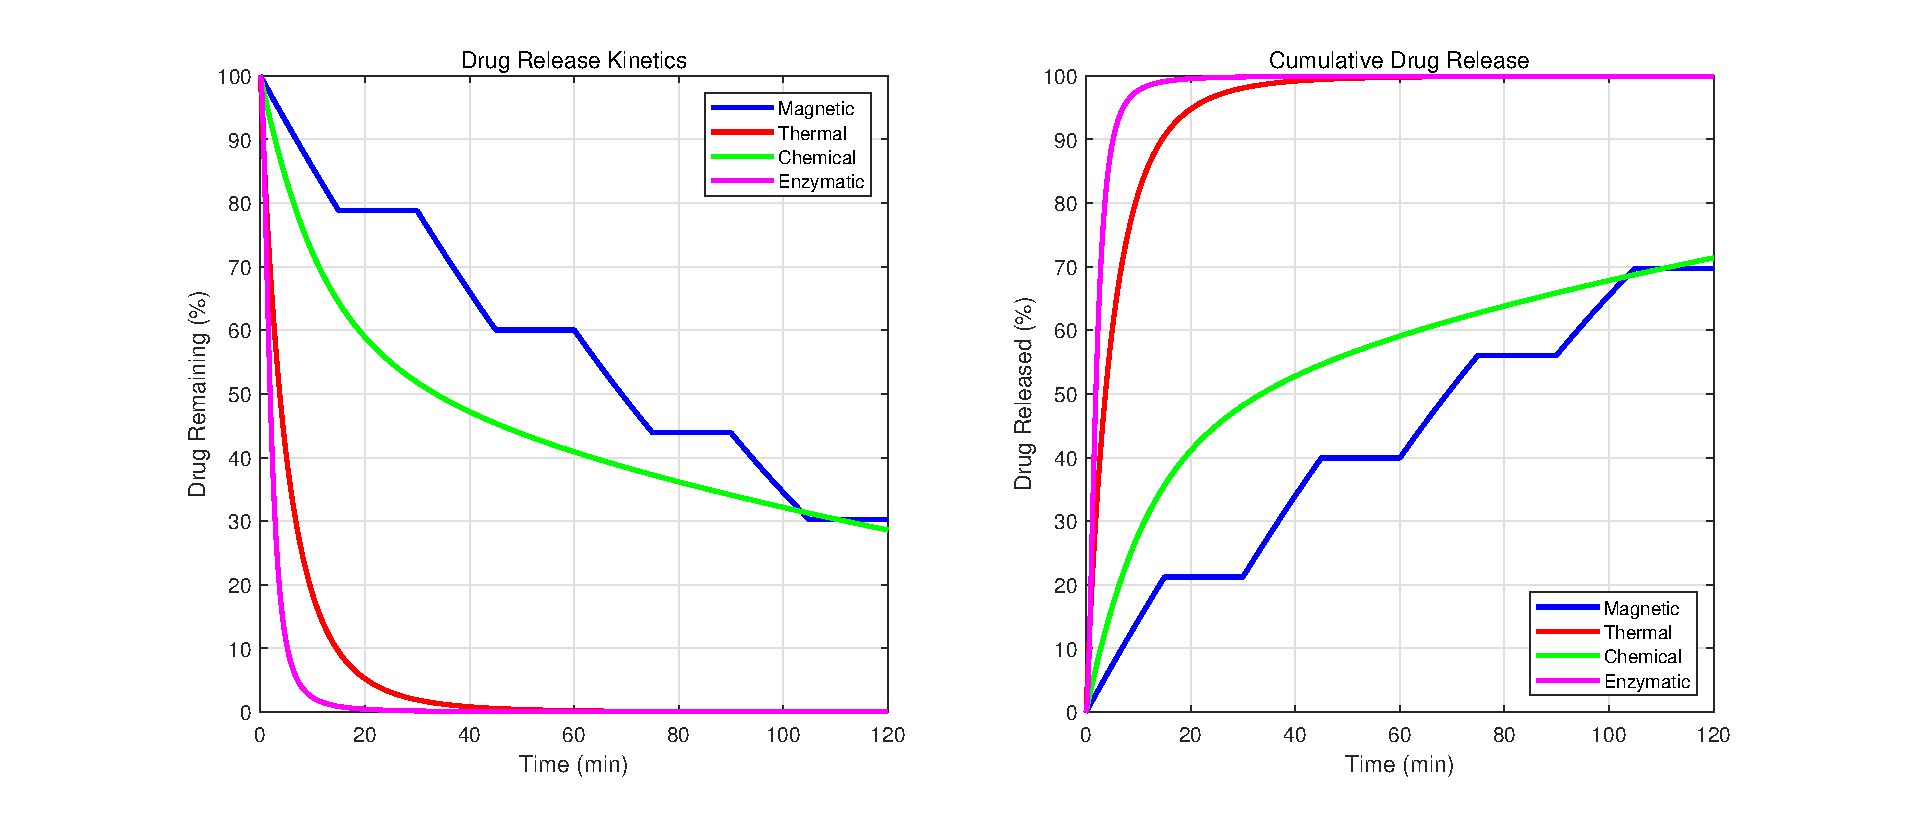
\includegraphics[width=4in]{DrugRelease.eps}
\end{minipage}
\hfill
  \begin{minipage}{2.4in}
\leftline{(b)}
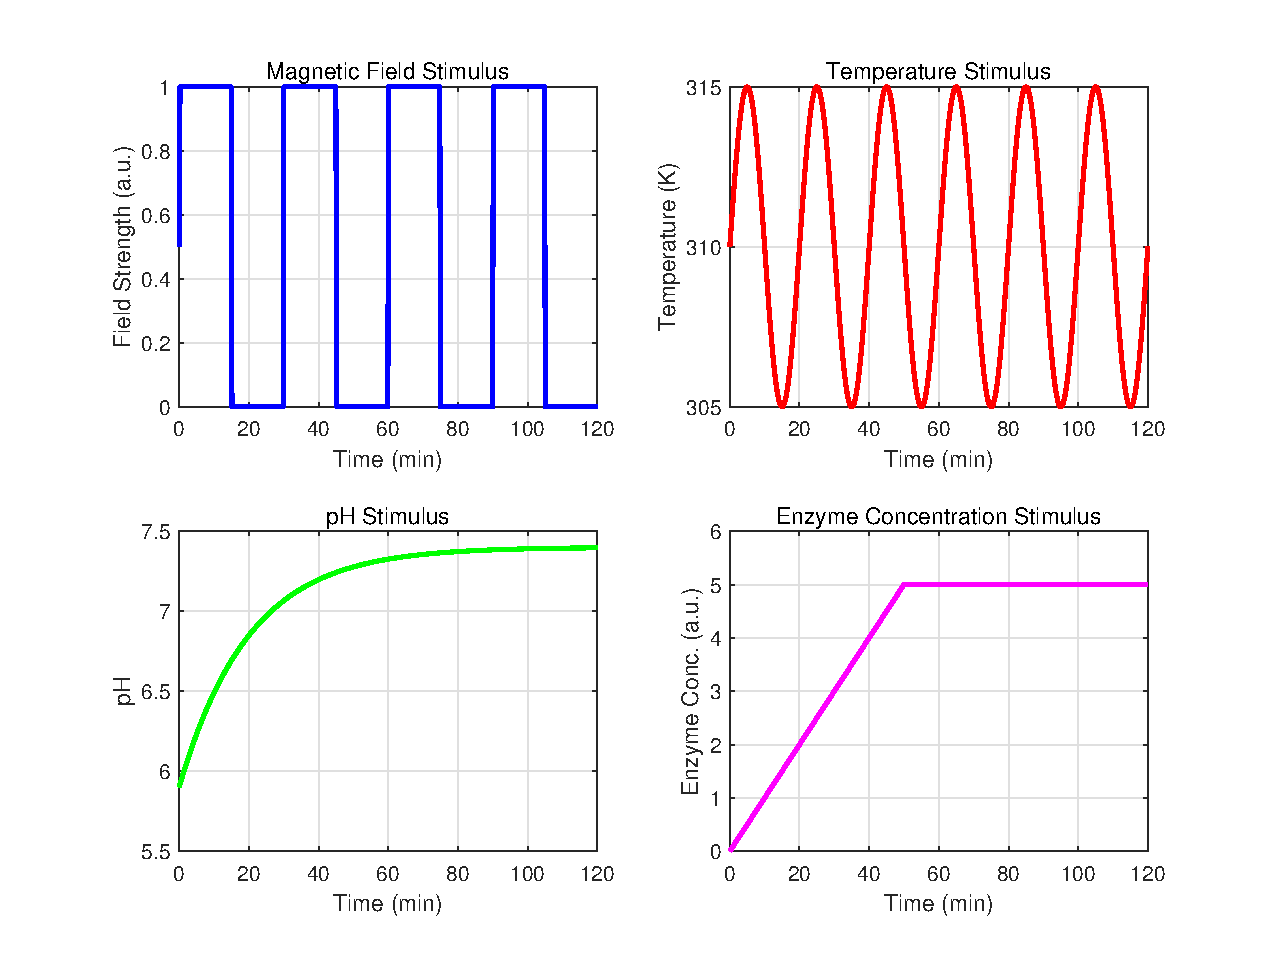
\includegraphics[width=2.4in]{MagneticField.eps}
\end{minipage}
\caption{A comprehensive view for stimuli-responsive drug release from micro-robots: (a) ; (b) .}\label{drugReleaseModel}	
\end{center}
\end{figure}

\begin{figure}[H]
\vspace*{1pt}
\begin{center}
\begin{minipage}{5in}
		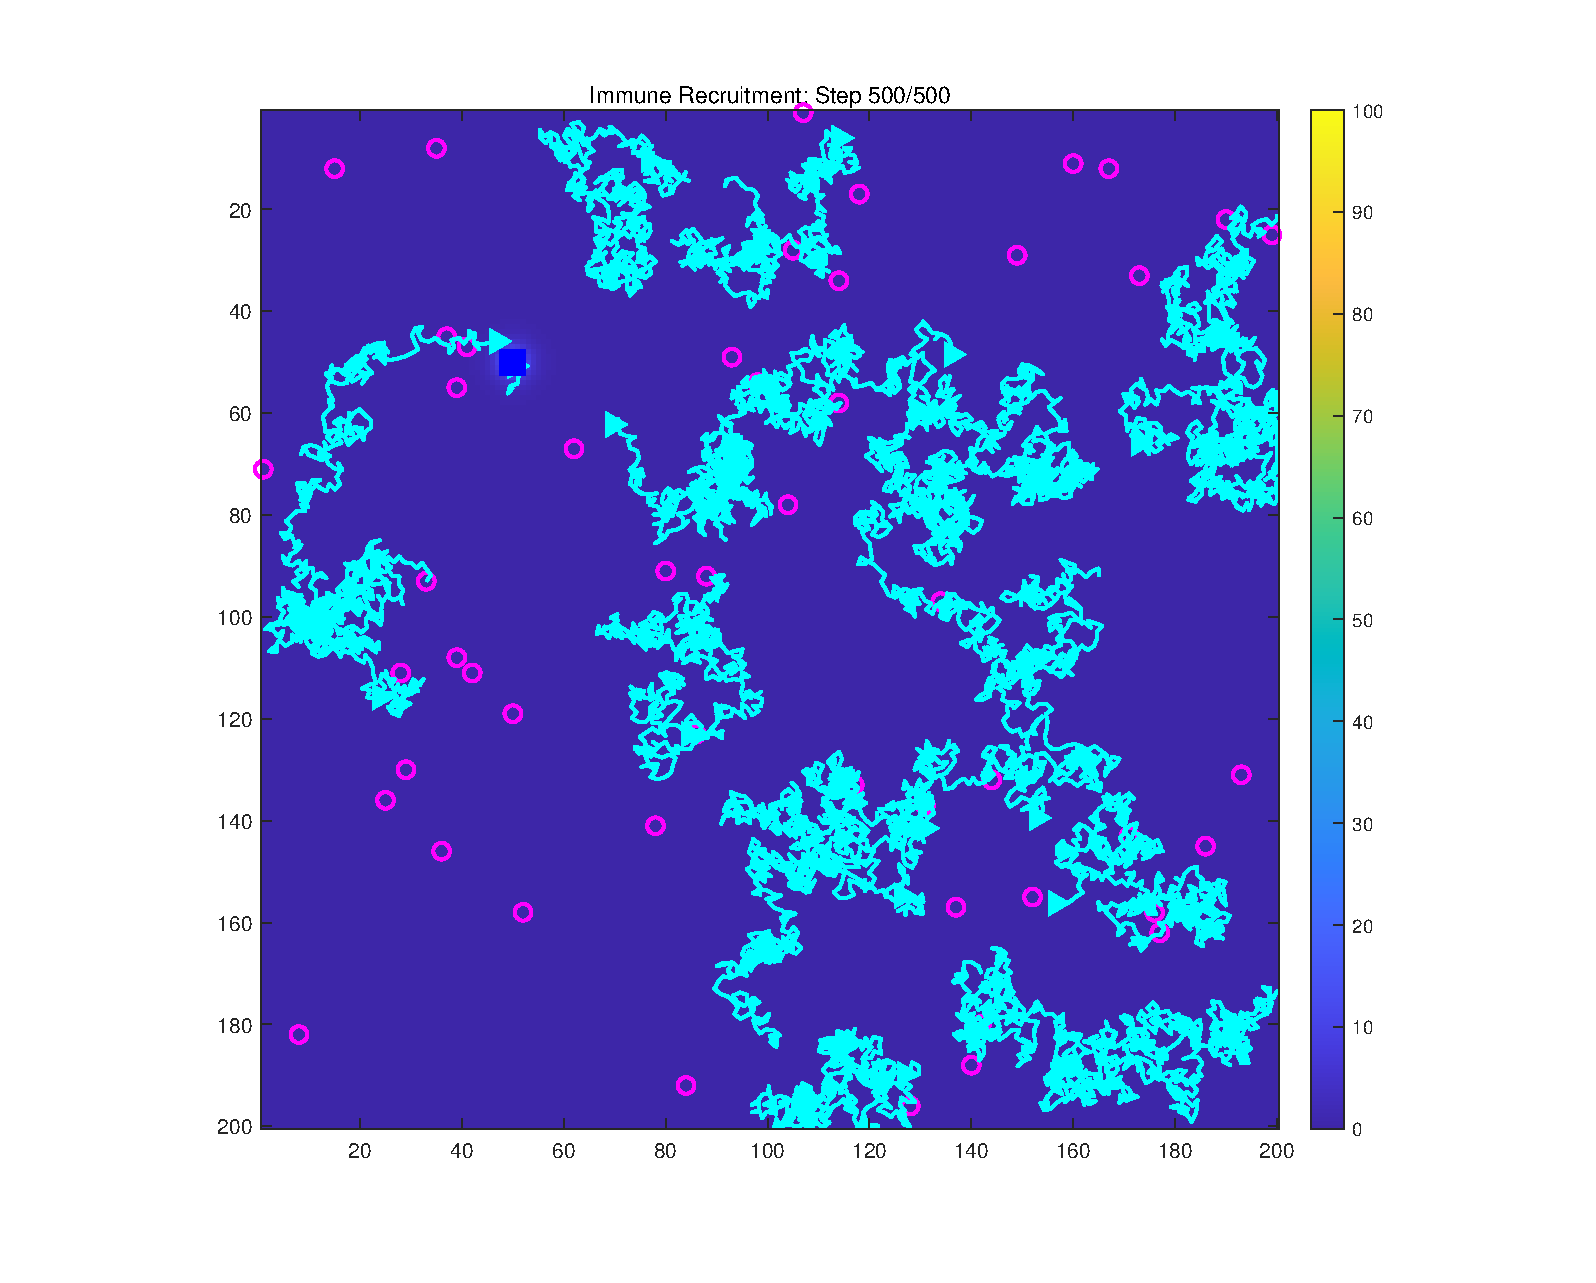
\includegraphics[width=5in]{ImmuneRecruitment.eps}
	\end{minipage}
\end{center}
\caption{}\label{immuneRecruitmentSim}	
\end{figure}
\section{Conclusions and future challenges}
Such studies are currently in progress and will be reported in future publications.
%\label{}

%This paper is organized as follows. In section 2, we present the framework for our random slow manifold reduction method for parameter estimation. Then in Section 3, we establish the error estimation for our parameter estimator in terms of observation error and slow reduction error by using analytical technique. Finally, we illustrate our estimation method numerically in a specific example.

%a specific example is tested to illustrate our estimation method in Section 4This paper is organized as follows. In section 2, we obtain an approximated random slow manifold and thus the random slow system. Then in Section 3, we establish the error estimation for our parameter estimator in terms of observation error and slow reduction error by using analytical technique. Finally, .
%% The Appendices part is started with the command \appendix;
%% appendix sections are then done as normal sections
%% \appendix

%% \section{}
%% \label{}

%% For citations use:
%%       \citet{<label>} ==> Jones et al. [21]
%%       \citep{<label>} ==> [21]
%%

%% If you have bibdatabase file and want bibtex to generate the
%% bibitems, please use
%%
%%  \bibliographystyle{elsarticle-num-names}
%%  \bibliography{<your bibdatabase>}

%% else use the following coding to input the bibitems directly in the
%% TeX file.




\renewcommand{\theequation}{\thesection.\arabic{equation}}
\setcounter{equation}{0}




\renewcommand{\theequation}{\thesection.\arabic{equation}}
\setcounter{equation}{0}



%\section*{References}

\bibliography{mybibfile}

\begin{thebibliography}{00}


\end{thebibliography}



\end{document}

\endinput
%%
%% End of file `elsarticle-template-num-names.tex'.
